\documentclass[../BTOF_summary.tex]{subfiles}
 
\begin{document}

\section{The \btof\ Detector Hardware}

The \btofD\ consists of 16 elements arranged symmetrically around the \panda\ interaction point. Each of these elements is called a \sm\ and comprises five main parts.

\begin{itemize}
	\item Active Medium (Scintillator Tiles)
	\item Photon Readout (\sipm)
	\item \sensorboard\ (flex PCB holding \sipms )
	\item Signal Transmission (PCB / \railboard )
	\item Enclosure (Carbon Fiber)
\end{itemize}

A single large PCB or a PCB split into a front and back part connect the Front End Electronics (FEE) to the detector elements. 
Each \sm\ is equipped with 60 scintillator tiles in two rows, read out by four \sipms\ on each side of the scintillator. 
This adds up to 3840 channels with a total amount of \num{15360} deployed \sipms .

\subsection{Scintillator}
Each scintillator of the \btofD\ is identical to the others and have the following dimensions; \SI{87 x 29.4 x 5}{mm}.
To fit inside the holding structure the corners of the scintillator tiles are truncated.
Each chamfer is set at \SI{3}{mm}.
This is a change from the design proposed in the Technical Design Report (TDR) which had rectangular scintillators.

The performance impact of this change was studied using a strontium source on a mechanized arm, comparing time resolution measurements of cut and uncut scintillator tiles.\todo[inline]{The measurements of Svetlana need to be integrated here}
As shown in \fig\ \todo{add figure} the bulk of the material shows little to no significant difference.
The time resolution of events in the corners... \todo{finish this paragraph}

\subsubsection*{Material}
The scintillator of choice for the detector dimensions is the EJ-232 by Eljen Technology. It is an organic scintillator compound developed for high accuracy timing applications \footnote{\url{https://eljentechnology.com/products/plastic-scintillators/ej-232-ej-232q}}.
The equivalent Saint-Gobain/Bicron equivalent product would be the BC-422 scintillator.
Another material candidate was the widely used EJ-228/BC-418.
It produces more photons but for the small dimensions of the \btof\ tiles delivers a slightly inferior time resolution.
%Due to the short emission wavelength the mean free path inside of the scintillator is only around \SI{10}{cm}.

Measurements comparing the scintillator thickness revealed stark differences in performance between \SI{3}{mm} and \SI{6}{mm} thick tiles. 
Under ideal circumstances, for equal readout surface and constant energy loss of passing particles, the number of detected photons is independent of the thickness.
However, since the number of internal reflections is increased for thinner tiles, more photons are lost at the scintillator surface compared to thicker modules.
This leads to a significant time resolution increase when reducing the tile thickness as can be seen in \fig ~\ref{fig:Tchickness_timeRes}.
Since the performance difference between \SIlist[]{5;6}{mm} is minimal and the material budget of the device needs to be kept at a minimum the detector will be equipped with \SI{5}{mm} thick tiles.

\begin{figure}[htbp]
	\centering
	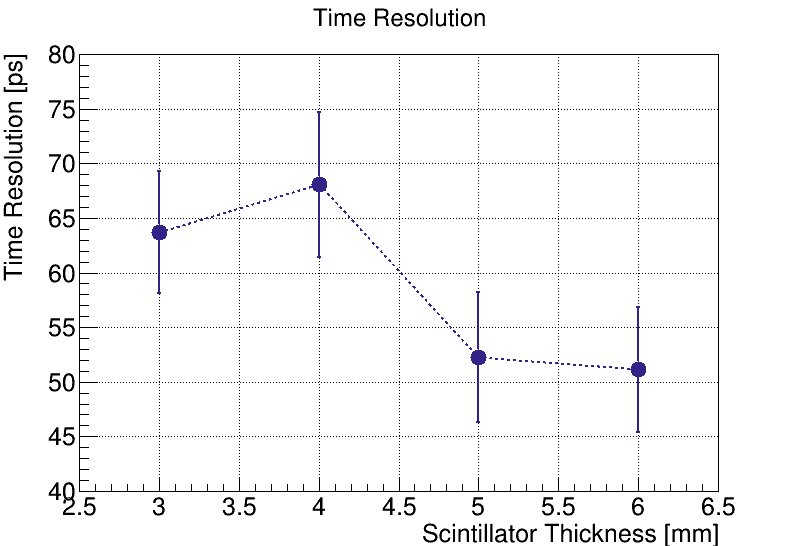
\includegraphics[width=.7\textwidth]{fig/TimeResSummary.png}
	\caption{Time resolution measurement comparing different thicknesses of aluminized mylar wrapped scintillator tiles.}
	\label{fig:Tchickness_timeRes}
\end{figure}

\subsubsection*{Wrapping}
Since the time resolution of a scintillator detector is coupled to the number of detected photons, the scintillator tiles are wrapped in order to reflect photons that escape the scintillator back into it.
The material choice was subject to tests performed on a scintillator tile using a \sr\ source in order to determine the best performing wrapping.
Material candidates were aluminized mylar foil, Tyvek hardstructure 1057D, enhanced specular reflector (ESR), Teflon tape, aluminum foil and no wrapping.
As can be seen in Table~\ref{tab:WrappingTest}, taken from the \btof\ TDR\todo[]{add Ref to TDR}, the performance difference was within \SI{6.7}{ps} from the best to the worst performing wrapping and a standard deviation of \SI{2.23}{ps}.

\begin{table*}[htbp]
	\caption[Time resolution for different wrapping materials]{Time resolution of EJ-232 (top) and EJ-228 (bottom) plastic scintillator tiles for various wrapping materials.
		\label{tab:WrappingTest}}
	\centering
	%\resizebox{0.8\textwidth}{!}
	{
		\begin{tabular}{ l  c  c }
			\toprule
			Wrapping material                 & Time resolution [ps] & Number of detected photons \\
			\midrule
			No wrapping                       & 55.0\,$\pm$\,0.3     & 288\,$\pm$\,2\\
			Aluminized Mylar foil             & 52.7\,$\pm$\,0.3     & 355\,$\pm$\,2\\
			Tyvek hardstructure 1057D         & 55.0\,$\pm$\,0.3     & 394\,$\pm$\,3\\
			Enhanced specular reflector (ESR) & 55.2\,$\pm$\,0.3     & 355\,$\pm$\,3\\
			Teflon tape                       & 59.4\,$\pm$\,0.3     & 408\,$\pm$\,4\\
			Aluminum foil                     & 54.2\,$\pm$\,0.3     & 344\,$\pm$\,3\\
			\midrule
		\end{tabular}
	}
\end{table*}

Surprisingly, Teflon tape, the by far worst performing wrapping, produced the largest amount of detected photons.
The best performing material and the only one better than no wrapping at all was the aluminized mylar foil.
This can be attributed to the type of reflection.
While aluminized mylar has a mirror like finish, the other materials produce diffuse reflections.
This leads to larger distances travelled by the photons before reaching the photo detectors.

The wrapping material of choice for the scintillator tile of the \btofD\ is aluminized mylar.


\subsection{\sipm}

To detect the photons produced in the scintillators a device is needed that fits into the limited space available to the detector, can operate within a strong magnetic field and delivers a good time resolution.
A sensor that fits these criteria is the Silicon Photomultiplier (\sipm ).
These small devices are available in multiple sizes.
Best suited for the \btofD\ is an effective photosensitive area of \SI{3x3}{mm} with a thickness in the order of \SI{1.5}{mm}.

Multiple manufacturers offer sensors of such kind including \hamamatsu, \ketek and \advansid\ each with slightly different operational parameters.
One main point to consider is the operational voltage which differs greatly between manufacturers.
While \hamamatsu\ \sipms\ are operated at around \SI{60}{V}, \ketek\ \sipms\ only require a bias voltage of around \SI{30}{V}.
Since the sensors will be connected in series as described in Section \todo{add section on SiPM serial connection}, the operational voltage is 4 times the single sensor voltage, which affects the requirements from necessary electronics to drive the sensors.

The final choice on which \sipm\ model to use has not been made since the development of \sipms\ moves relatively fast and new product generations were expected.
Tested sensors include the \texttt{S13360-3050PE} by \hamamatsu, the \texttt{PM3350} by \ketek\ and the \texttt{ASD-NUV3S-P} by \advansid , which all perform adequately.

\subsubsection*{Serial connection of 4 \sipms}

In order to effectively readout the \SI{5x30}{mm} large surface area of the ends of the scintillator tile, the active surface needs to be extended beyond a single \sipm\ with an effective photosensitive are of \SI{3x3}{mm}.
To do this four \sipms\ are connected in series.
This offers a larger active area without increasing the detector complexity by adding unnecessary channels by reading out the \sipms\ individually.

Additionally connecting the sensors in series in contrast to a parallel connection, offers an improvement of the signal timing properties.
The slope of the rising signal flank, which determines the signals timing susceptibility to electrical noise, depends on the sensors internal capacitance.
A smaller capacitance leads to a faster sensor discharge and a steeper signal slope.
Connecting the sensors in series decreases this internal capacitance making the signal faster whereas a parallel connection would have the opposite effect.

There is evidence suggesting, that increasing the amount of \sipms\ from 4 to 6 would improve the time resolution.
These tests however were performed at a time where the scintillator was held in place differently and hence was not chamfered.
Cutting away \SI{3}{mm} from either edge reduces the available space to \SI{24}{mm}.
With the actual width of each \sipm\ is slightly below \SI{4}{mm} and an LED between the middle two sensors, there simply is not enough room for additional sensors.

\subsection{\sensorboard}

To connect the \sipms\ to the readout they are soldered onto a flex PCB called the \sensorboard .
It not only holds the photon sensors but also the temperature sensor and a calibration LED.
To establish a secure connection between the \sipms\ and the scintillator it is glued onto the scintillator tile as seen in \fig~\ref{fig:SensorBoradNew}.

\begin{figure}[htbp]
	\centering
	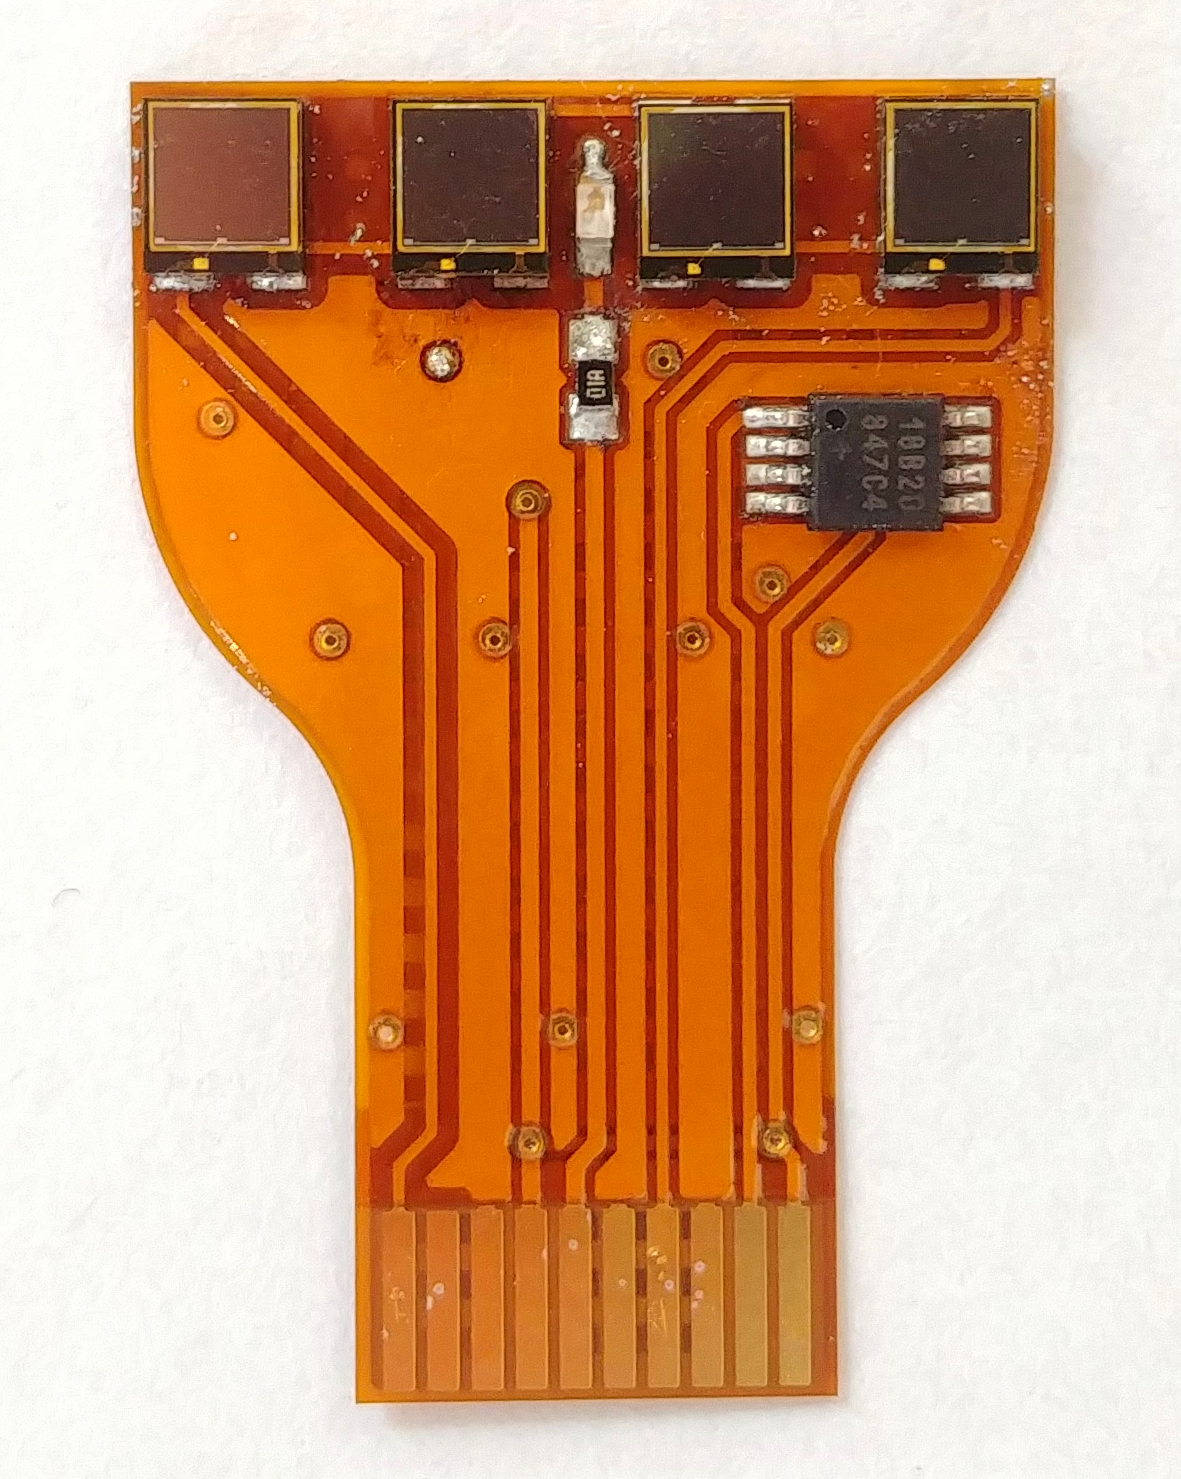
\includegraphics[height=5cm]{fig/SensorBoardNew2.png}
	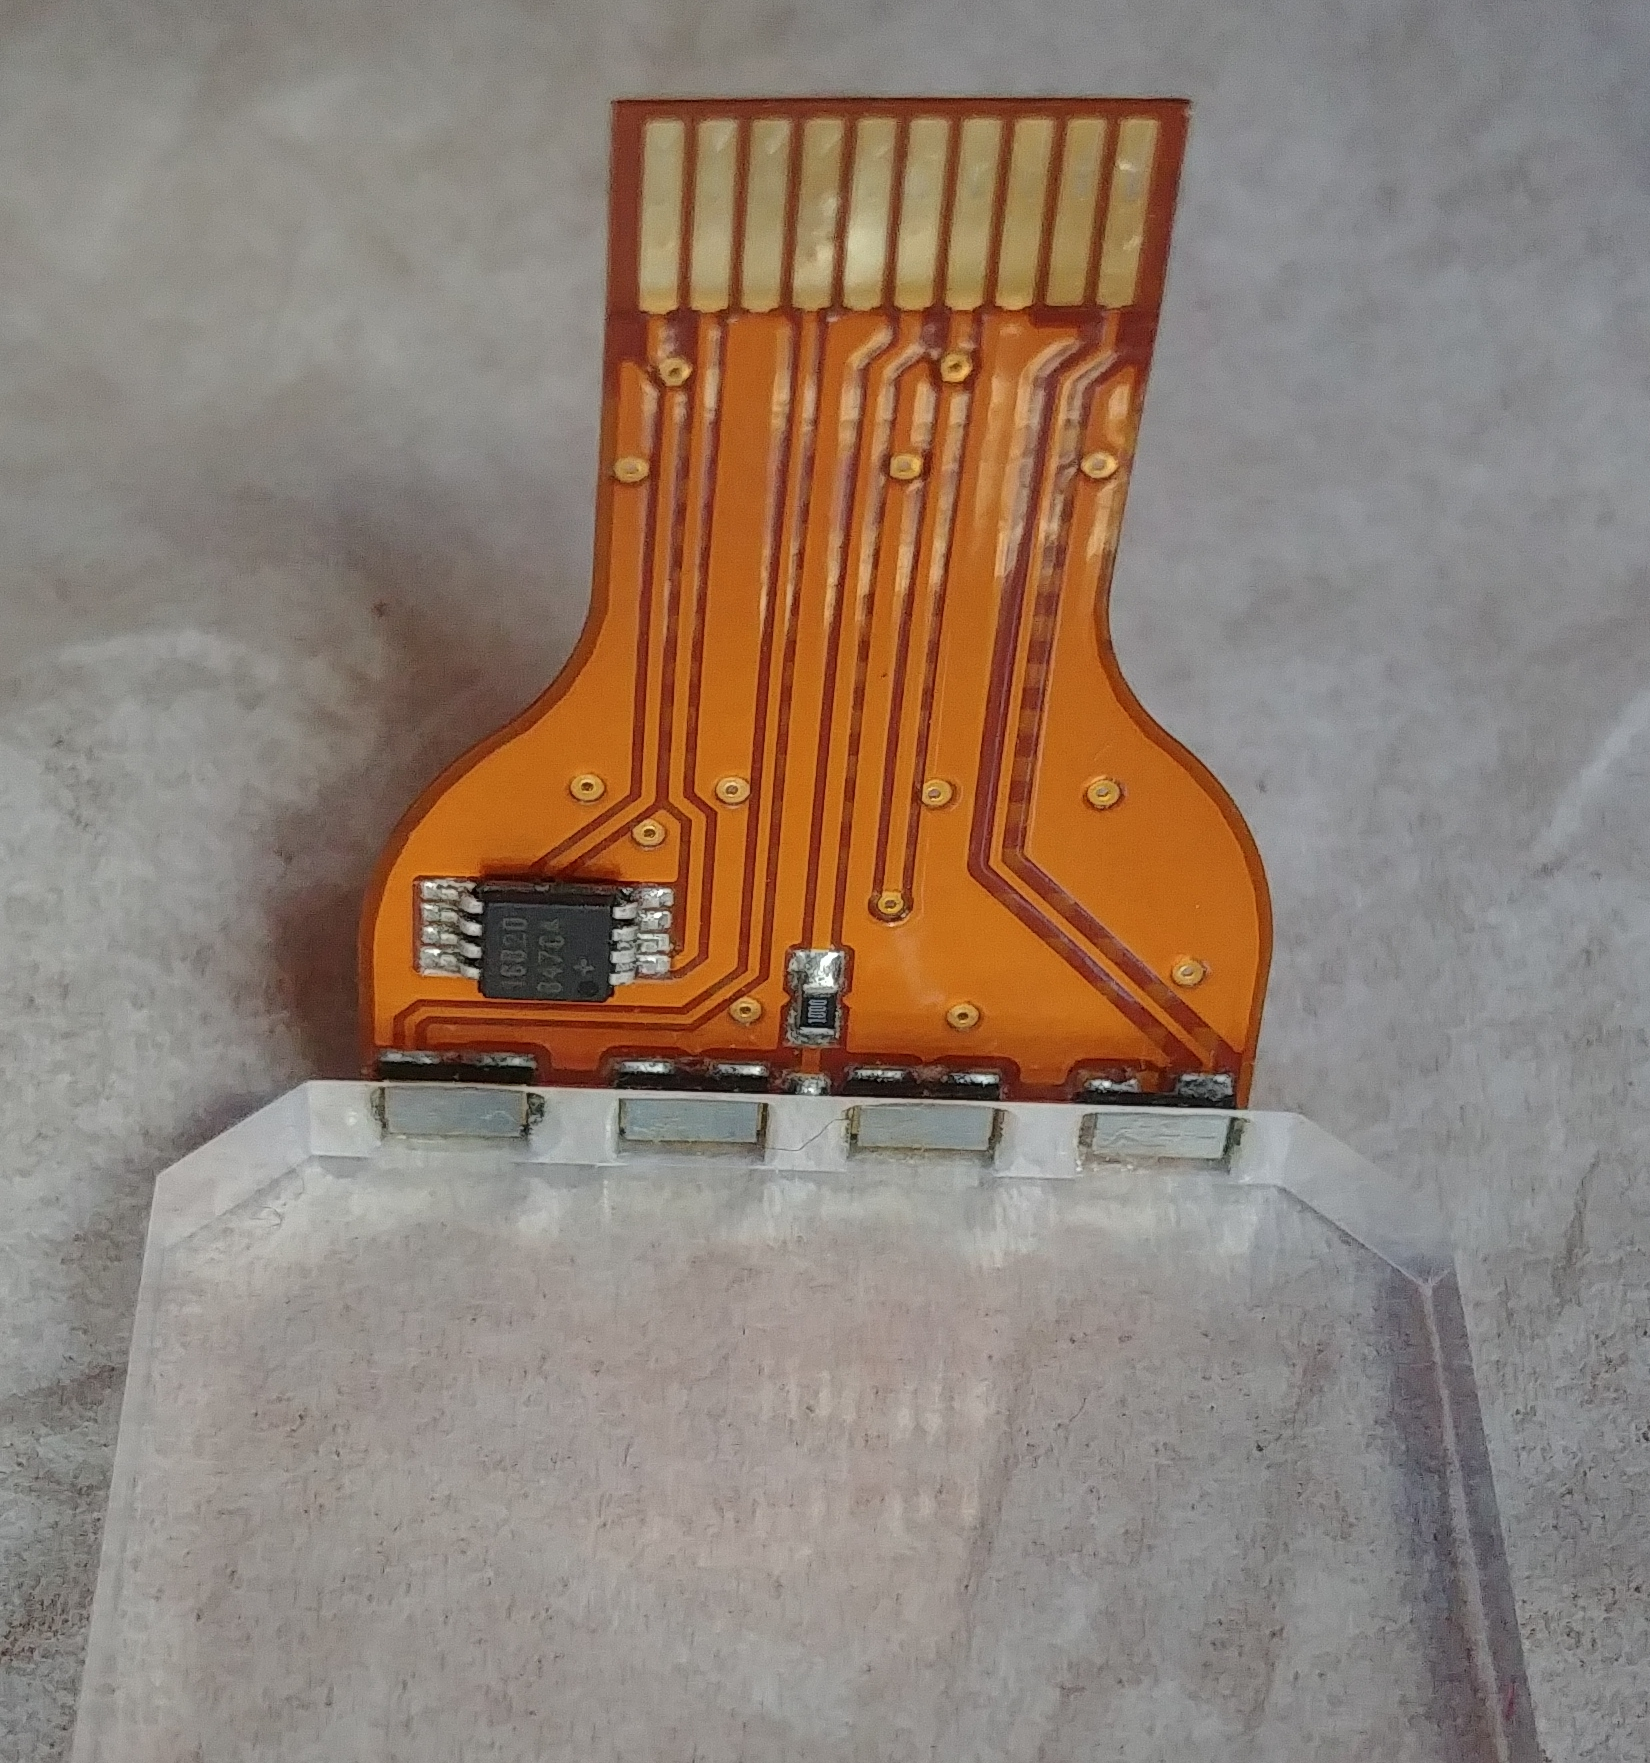
\includegraphics[height=5cm]{fig/Sensorboards2Scintillator.jpg}
	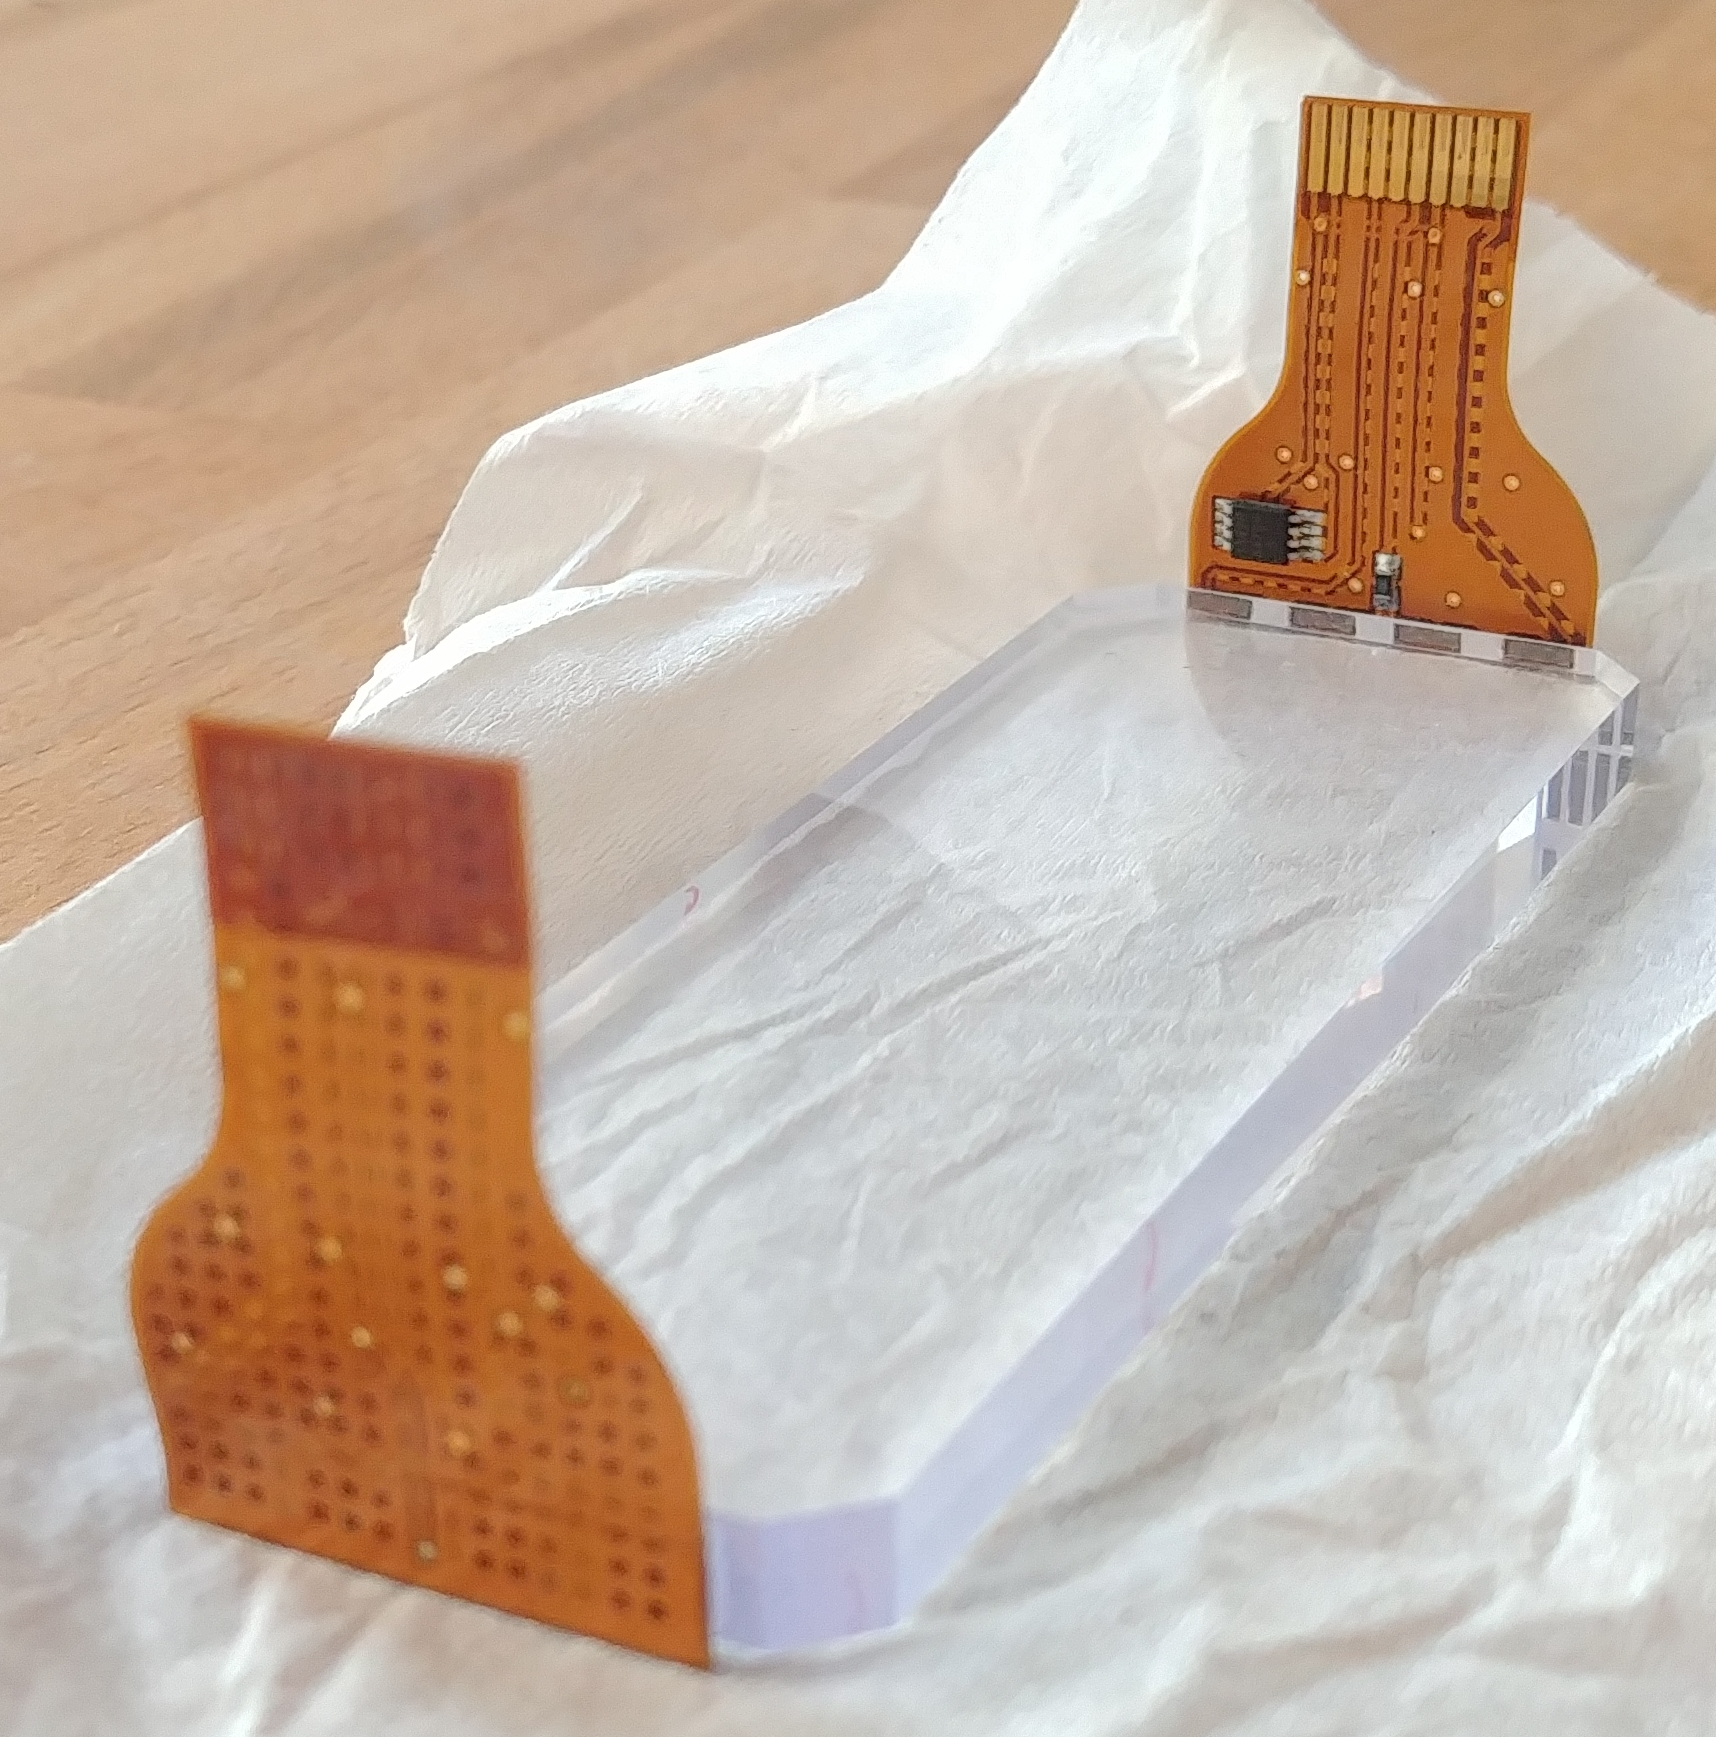
\includegraphics[height=5cm]{fig/Sensorboards2Scintillator2.jpg}
	\caption[The flexible \sensorboard .]{A flexible \sensorboard\ featuring four \sipms\ in series, a temperature sensor and an LED (left), attached to a scintillator (middle) and a full active module (right).}
	\label{fig:SensorBoradNew}
\end{figure}

The LED is supposed to function as a calibration and monitoring device during the operation of the detector.
Calibrated signals are produced by flashing the LED and any change in amplitude or time resolution can be picked up and monitored for changes.
The development of this procedure was subject of the work of a masters student who however never finished.
Since then the first idea has not been developed.

It would be necessary to determine the best way to drive the LEDs in order to produce a short and well defined signal. 
This includes the optimal voltage and duration of the driving signal, as well as determining what LED specifically would be optimal.
In general it is best to keep the emitted wavelengths as close to the scintillator light as possible to monitor the relevant performance.
Ultimately this development would need to be made in combination with finalizing the electronics for whole system.

Important findings during the testing of this new board is that the thin copper lines are very fragile.
Multiple strong bends can sever the connection between the \sipms\ and the \railboard .
For this reason it is important to handle these boards with care.
To remedy this the transition of the \sipm\ solder pad to the transmission line was changed from a strict \ang{90} corner to a smoother teardrop shaped junction.\todo[]{add info on how this change affected the reliability of the boards}
\todo[inline]{the first version of these boards what not propperly impedance matched. The second version should be by increasing transmission line width and adding a copper back plane.}

%%%%%%%%%%%%%%%%%%%%%%%%%%%%%%%%%%%%%%%%%%%%%%%%%%%%%%%%%%%%%%%%%%
\subsubsection{Temperature Sensor}
In order to monitor the climate the scintillator tiles and the \sipms\ are subject to, every sensor board is equipped with a temperature sensor. It was important that these devices can be read out using a minimal amount of channels or transmission lines to keep the material budget and \railboard\ occupancy at a minimum.
An individual channel for all 240 \sensorboard s per \sm\ would also overload the readout system.

A solution to this is a digital temperature sensor on a 1-Wire bus.
This bus offers the capability to connect a large amount of sensors in parallel, only requiring a ground, signal and power supply line.
Such a sensor which is used on the \sensorboard s is the \texttt{DS18B20} by \textit{Maxim Integrated}.
These sensors can be controlled by a micro controller and utilize a hard coded 48-bit address for each sensor, which far exceeds the number of necessary sensors for one \railboard .
To power them a bias voltage between \SIrange[]{3}{5.5}{V} is required.
A schematic of the connection of such sensors can be seen in \fig ~\ref{fig:DS18B20_connection}.

\begin{figure}[htbp]
	\centering
	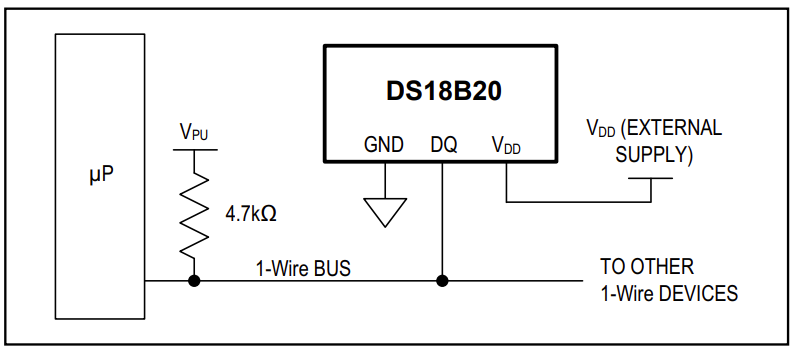
\includegraphics[width=.6\textwidth]{fig/DS18B20_connection.png}
	\caption[Connection scheme for the DS18B20 temperature sensor.]{Connection scheme for the DS18B20 temperature sensor connected to a micro processor (µP).}
	\label{fig:DS18B20_connection}
\end{figure}

\todo[inline]{add more info from Bernds thesis concerning function of the sensor. How long does it take to read out, etc}


\subsection{\railboard}

The solution to connect the photo sensors to the FEE and provide mechanical support at the same time is the \railboard .
It is a long PCB split into two parts due to availability issues of the base material.

Previous designs relied solely on the mechanical support of a single \railboard\ spanning the entirety of a \sm\ to hold all components including the scintillators in place.
Due to stability issues and too small tolerances in the connectors the form of the board has been redesigned and a carbon frame has been added.
The single \railboard\ is replaced by four large PCB's, one of which is shown in \fig ~\ref{fig:Railboard}.
Two of these boards are attached by ribbon cables to connect one full row of 60 scintillators to the FEE and held in place by plastic screws to the carbon frame.

\begin{figure}
	\centering
	\includegraphics*[width=.9\textwidth]{fig/Railboard3_imageCombined.png}
	\caption{Combined depiction of the internal transmission line layout and a photograph of the front part of the \railboard .}
	\label{fig:Railboard}
\end{figure}

Each board consists of 16 conductor layers alternating between shielding ground layers, which span the almost the entire layer and signal transmission lines, which can be seen in \fig ~\ref{fig:Railboard3_schematic}.
Since resistive losses at the relevant frequencies are dominated by the skin effect it is necessary to keep the conductor surface as large as possible.
In order to maximize the conductor surface while minimizing the material budget all conductor layers are kept as thin as possible with a thickness of \SI{17}{\micro \meter}.
For the purposes of minimizing reflection losses, the characteristic impedance of the whole board was kept around \SI{50}{\ohm}.
For this the relation between the width of the transmission lines and the substrate thickness had be calculated.
Since vertical space is limited a laminate thickness of \SI{0.406}{mm} was chosen which mandates a transmission line width of \SI{400}{\micro m}.

\begin{figure}
	\centering
	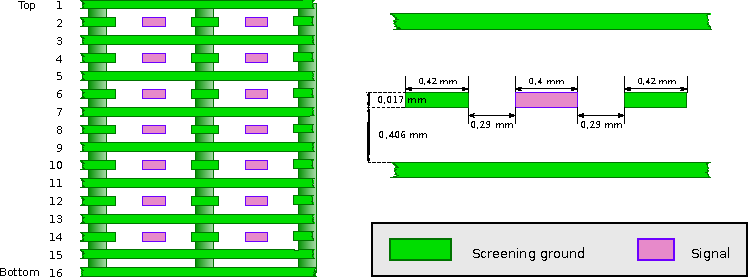
\includegraphics[width=.9\textwidth]{fig/Railboard3_schematic.pdf}
	\caption{Schematic of the internal layout of the \railboard\ conductors. The board substrate material is left blank.}
	\label{fig:Railboard3_schematic}
\end{figure}

% low loss material
\sipm\ signals with a rise time of \SI{3}{ns} correspond to a frequency of \SI{167}{MHz}.
At this frequency dielectric losses start to take on a larger portion of the electric losses experienced along a transmission line\footnote{more information in the dissertation "Development of the Fast Timing \panda\ Barrel Time-of-Flight Detector" by S. Zimmermann}.
To reduce these losses special PCB substrate materials have been developed such as RO4003C by Rogers Corp.
This is the material that is used for the \btof\ \railboard\ to ensure minimal losses for an optimal performance.
Since RO4003C sheets are not available beyond 48 inches or \SI{1.224}{m} the boards need to be split into a front and back part each holding 30 scintillators.
The mentioned size is the standard sheet size.
We did not make inquiries to determine whether larger nonstandard sizes were available.
Since the board is split already and requires external support it only makes sense to separate the scintillator rows along the long axis.
This gives the detector a higher degree of modularity and makes installation and swapping of components easier.

%%%%%%%%%%%%%%%%%%%%%%%%%%%%%%%%%%%%%%%%%%%%%%%%%%%%%%%%%%%%%%%%%%%%%%%%%%%%
\subsection{Connectors}

The board is equipped with three types of connectors, that 
\begin{enumerate*}[I) ]
	\item  connect the two halves of the \railboard\ to one another, 
	\item the \sensorboard s to the \railboard\ and 
	\item establishes a connection between the \railboard\ and the TOFPET ASIC.
\end{enumerate*}\todo[]{maybe make this a bulleted list for better readibility.}

\textbf{I)} The connectors for the ribbon cables between the boards as well as the connectors for the \sensorboard s are FFC/FPC\footnote{Flex Flat Cable / Flex Printed Circuit} connectors.
To connect the two \railboard halves, as shown in \fig ~\ref{fig:Railboard_connection} two distinct FFC connectors are used.
Transmission lines which carry detector signals are connected via the \texttt{FH28-60S-0.5SH} connector by Hirose Electric Group, which is depicted in \fig~\ref{fig:Railboard_connector}.
Connections for the power delivery and the temperature sensors are connected using the \texttt{ZF1-25} by Samtec, shown in \fig~\ref{fig:Railboard_power_connection}.
The main difference between the two connectors is the pitch size of connectors pins.
Since there are many more signal lines on the \railboard\ than power lines, these have higher pitched connectors.
If the number of power lines is to be increased this could be changed.
It however is important to keep in mind that the higher the pitch of the connector, the closer each line is to one another physically limiting the voltage it can successfully sustain.
\todo[inline]{add picture of cable and connectors.}

\begin{figure}
	\centering
	\includegraphics[width=.7\textwidth]{fig/Railboard_Connection_filter.png}
	\caption{Connection between the \railboard\ halves.}
	\label{fig:Railboard_connection}
\end{figure}

\begin{figure}
	\centering
	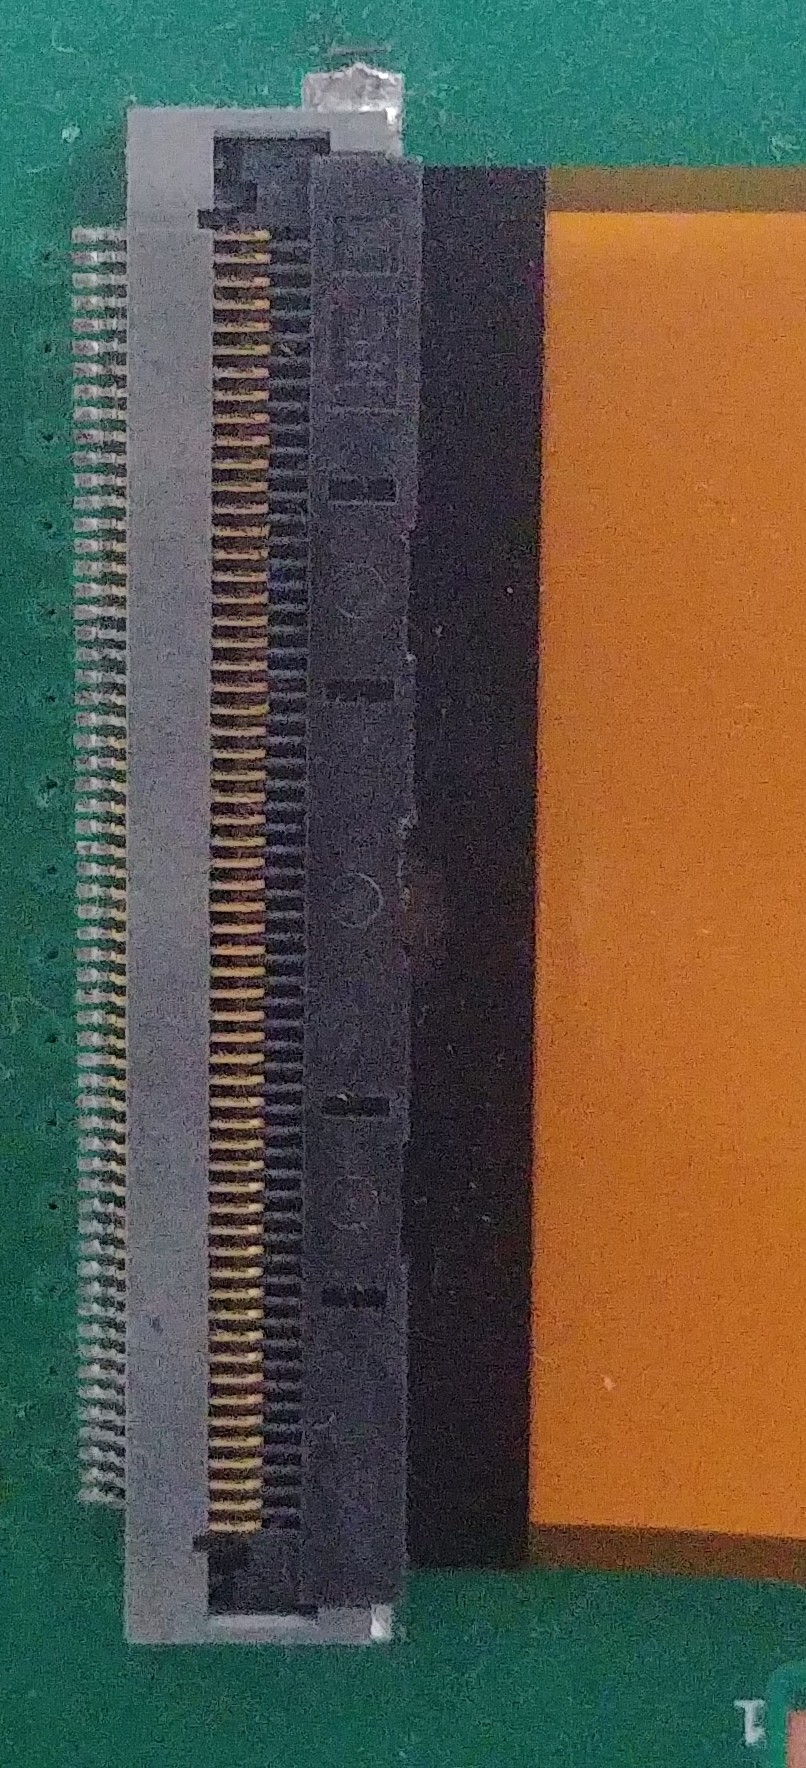
\includegraphics[height=5cm]{fig/LargeConnector_cable_crop.jpg}
	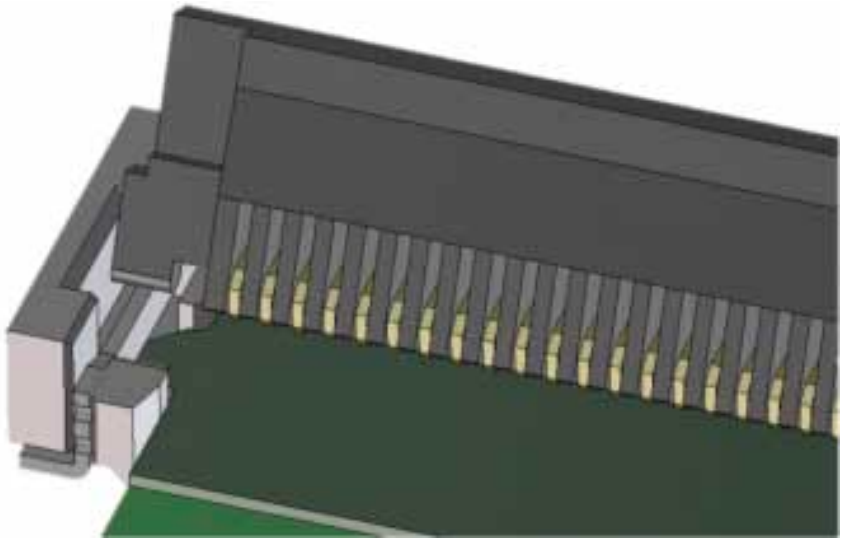
\includegraphics[height=5cm]{fig/hirose_connector_drawing.png}
	\caption{Foto and drawing of the \railboard\ connector for the ribbon cable between boards.}
	\label{fig:Railboard_connector}
\end{figure}

\begin{figure}
	\centering
	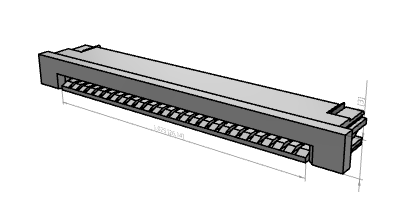
\includegraphics[height=5cm]{fig/Connector_ZF1-25-01.png}
	\caption{Connector for power between \railboard s.}
	\label{fig:Railboard_power_connection}
\end{figure}

\textbf{II)} Similar connectors are used for the \sensorboard s. These are also connected via flat ribbon cable connectors. The model used is a zero insertion force connector by Samtec (\texttt{ZF1-10-01-T-WT-TR}) depicted in \fig~\ref{fig:SensorBoard_connector} with a naked \sensorboard .
To open the connector the black plastic tab is pulled out.
After the \sensorboard\ is inserted or extracted the black tab is pushed closed to fasten the board inside and establish a secure connection.
\todo[inline]{add more info on the connectors.}

\begin{figure}[htbp]
	\centering
	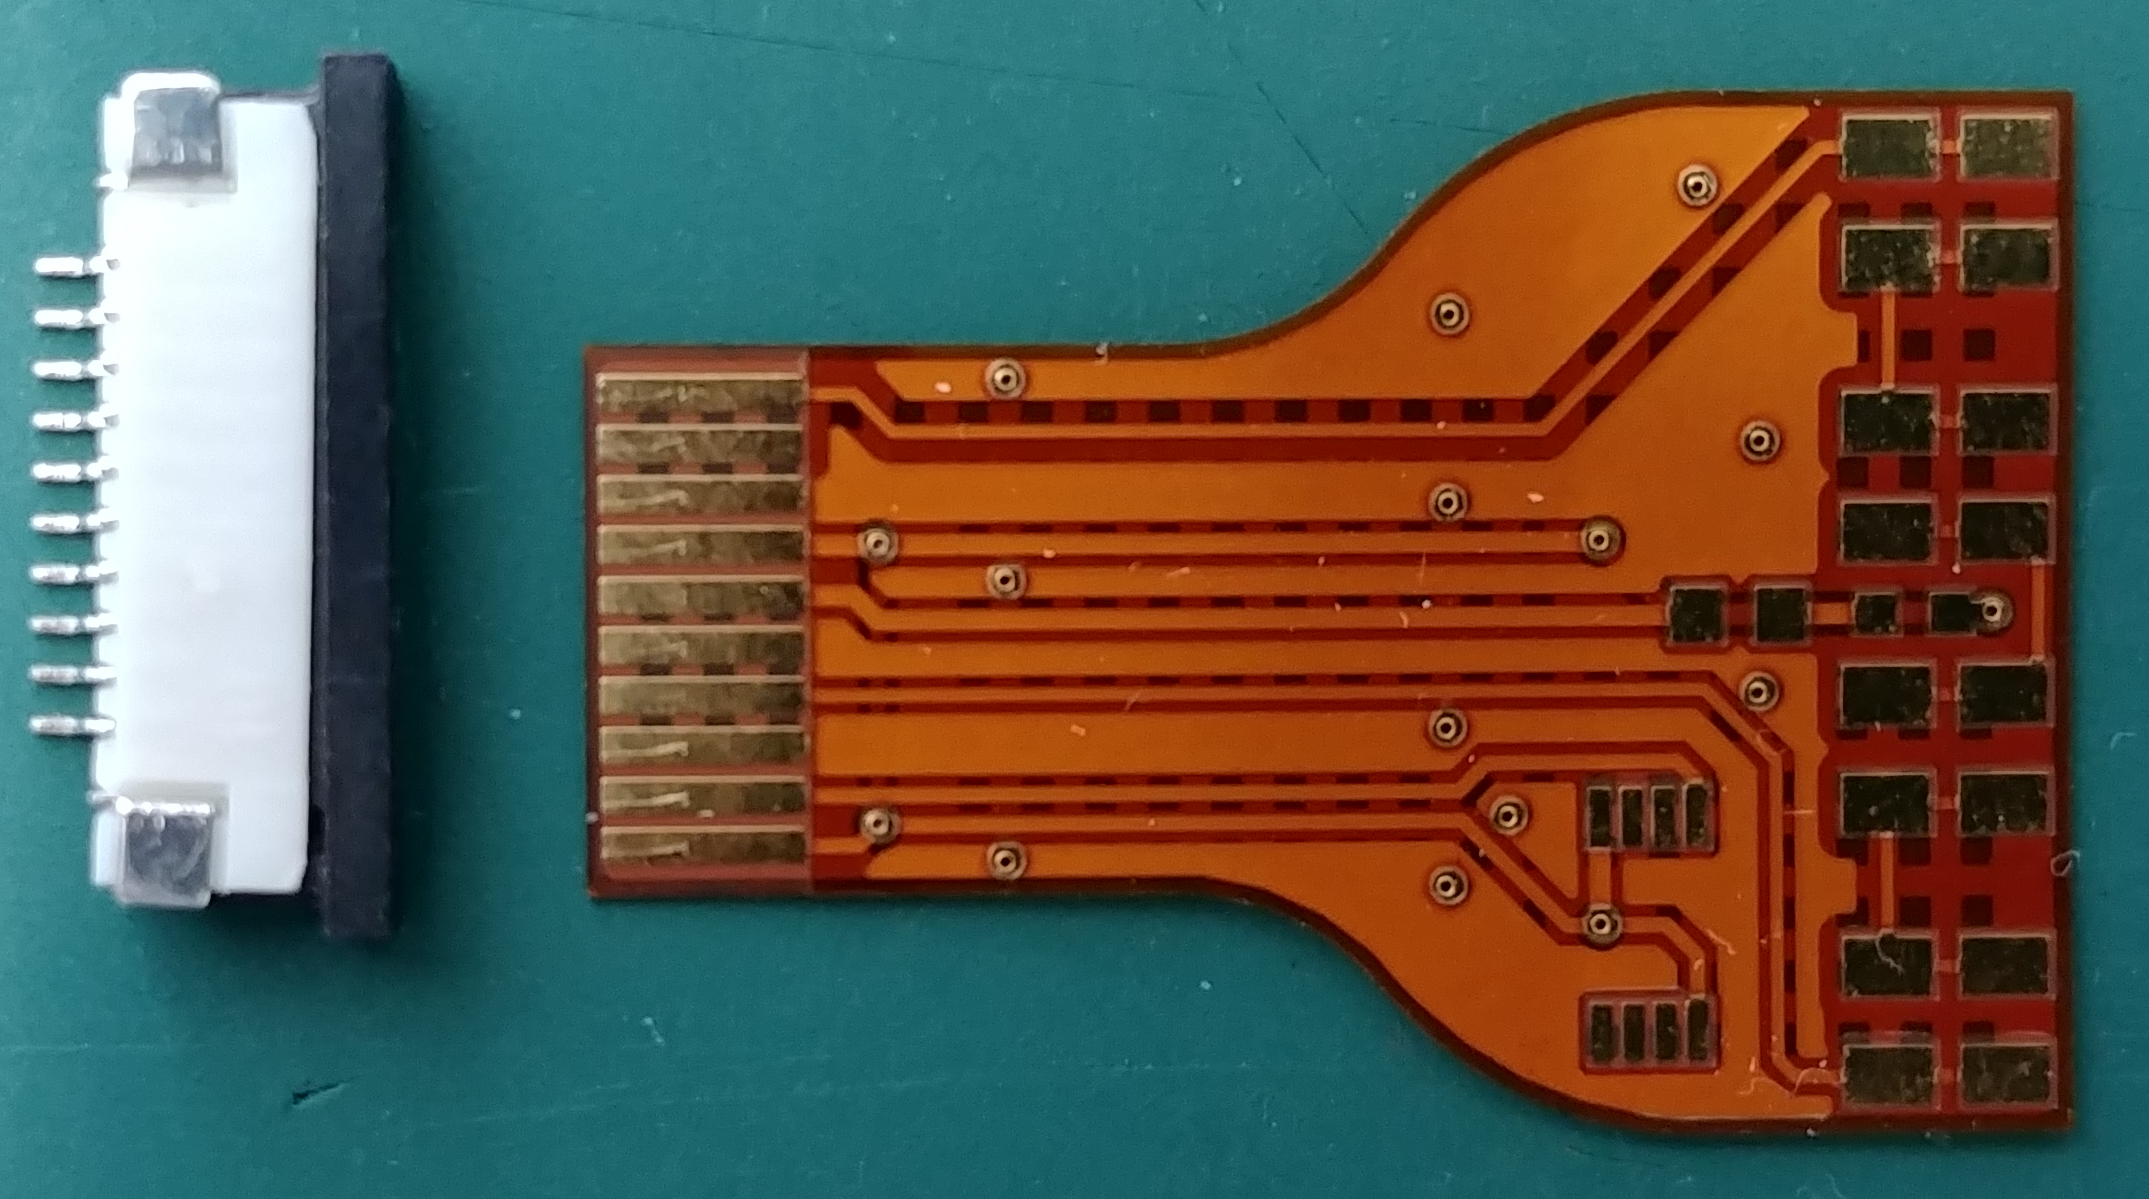
\includegraphics[width=.5\textwidth]{fig/SensorBoard_connector.png}
	\caption{Zero insertion force connector by Samtec used to connect the depicted \sensorboard\ to the \railboard .}
	\label{fig:SensorBoard_connector}
\end{figure}

\textbf{III)} The connection to the FEE has not been decided on yet since the FEE itself is not final.
The concept however is to use the connectors the PETsys boards use natively to attach them to the \railboard\ directly.
In the mean time small \texttt{MMCX} connectors are being used to quickly attach an oscilloscope or other devices such as preamps to the transmission lines.



\end{document}